Il seguente codice MatLab contiene l'implementazione della \textit{spline} cubica interpolante (naturale o \textit{not-a-knot}, come specificato in ingresso) delle coppie di dati assegnate. La forma della funzione è del tipo :\\ \textit{y = spline3( xi, fi, x, tipo )}.\\\
\lstinputlisting[language=Matlab]{Cap_4/Es_5/spline3.m}
Da come si può vedere, all'interno del codice vengono richiamate le seguenti funzioni:\\\ 
\begin{itemize}
	\item \textbf{dd = differenzaDivisa(xi, fi)}
	      \lstinputlisting[language=Matlab]{Cap_4/Es_5/differenzaDivisa.m}
	\item \textbf{mi = risolviSistSplineNotAKnot(phi, xi, dd)}\\\
	      \lstinputlisting[language=Matlab]{Cap_4/Es_5/risolviSistSplineNotAKnot.m}
	\item \textbf{mi = risolviSistSplineNaturale(phi, xi, dd)}\\\
	      \lstinputlisting[language=Matlab]{Cap_4/Es_5/risolviSistSplineNaturale.m}
	\item \textbf{s = esprSpline3(xi, fi, mi)}\\\
	      \lstinputlisting[language=Matlab]{Cap_4/Es_5/esprSpline3.m}
	\item \textbf{y = valutaSpline(xi, s, x)}\\\
	      \lstinputlisting[language=Matlab]{Cap_4/Es_5/valutaSpline.m}
\end{itemize}

. \\ \\ Sotto un esempio di utilizzo per interpolare la funzione $y = \frac{1}{1+x^2}$ 
\lstinputlisting[language=Matlab]{Cap_4/Es_5/Es_5.m}


\begin{figure}[!ht]
	\makebox[\textwidth]{
		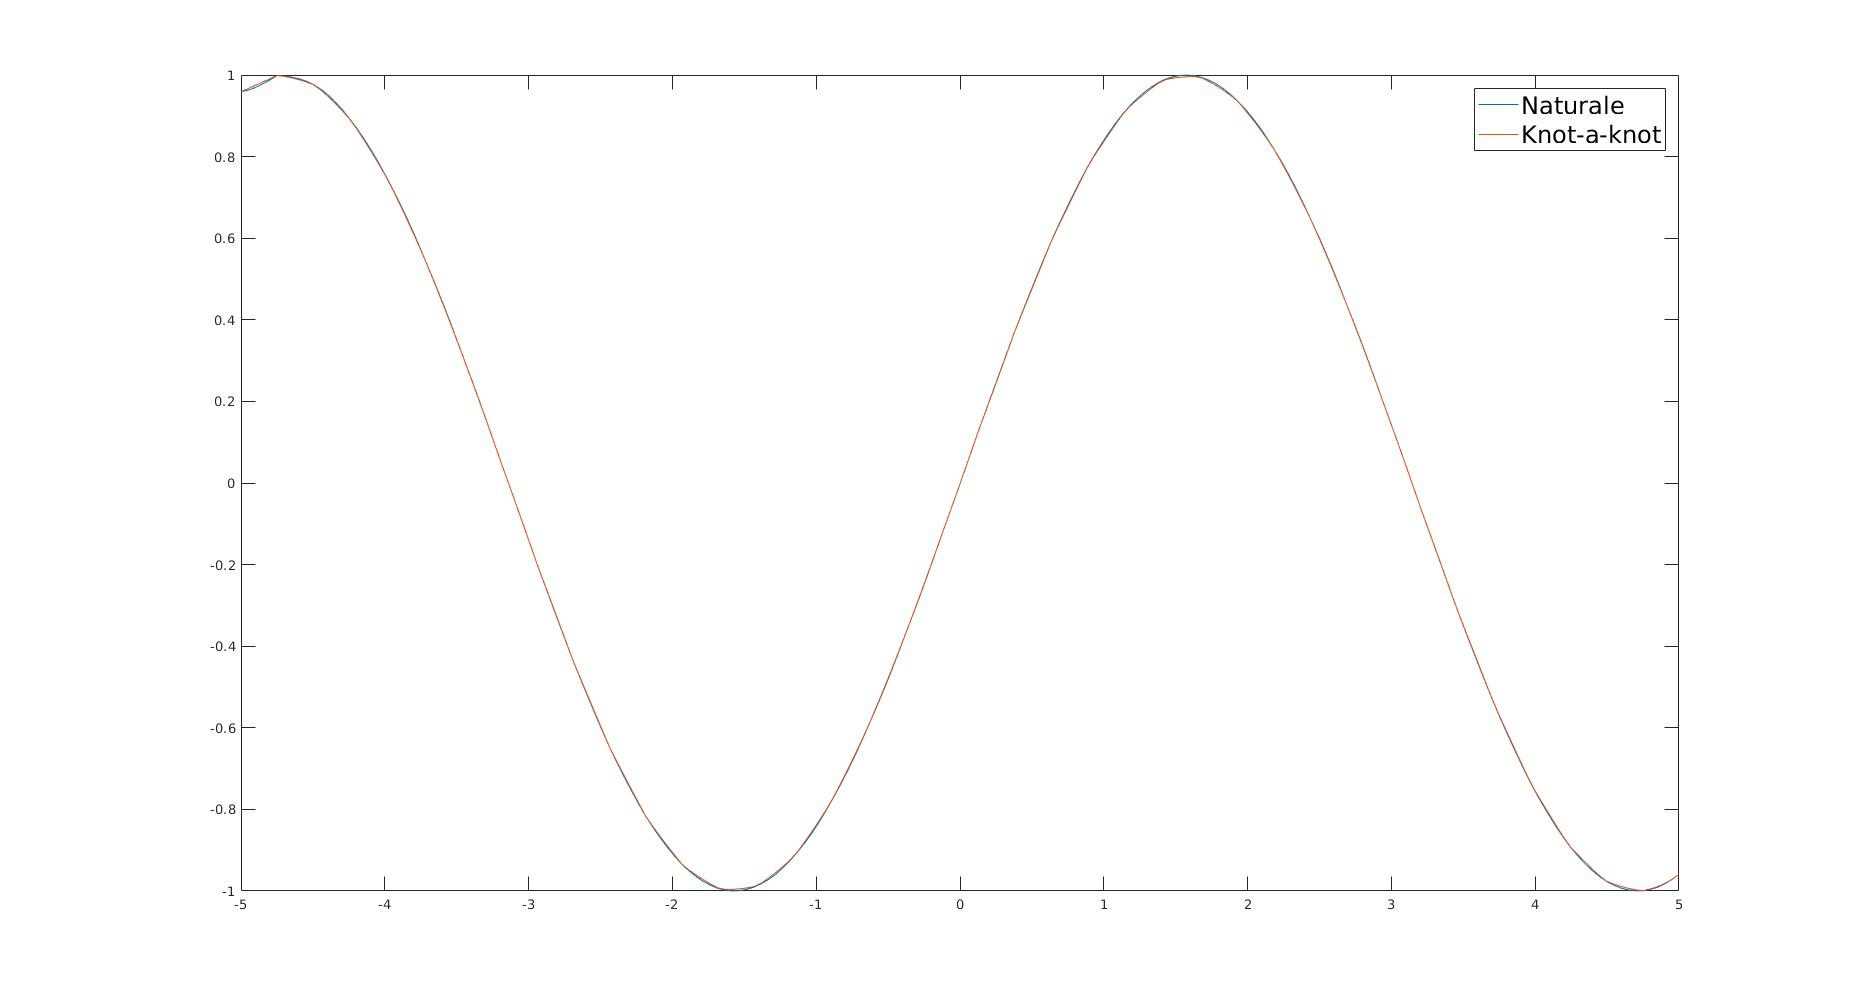
\includegraphics[width=\paperwidth]{Plot/Cap_4_Es_5}
	}
	\caption{Plot spline cubiche per $y = \frac{1}{1+x^2}$ }\label{fig:Cap_4_Es_5}
\end{figure}
